\section{}
\textit{Consider creeping flow of a sphere of diameter $D$ moving through a fluid at speed $V$. We gave an expression for drag force, $F_D = 3\pi\mu VD$. The drag coefficient $C_D$ over three-dimensional bodies is typically defined as $C_D = \frac{F_D}{\frac{1}{2}\rho V^2A}$, where $A$ is the frontal area of the body (the area you “see” when looking at the body from upstream). Generate an expression for $C_D$ in terms of Reynolds number for this flow.}

\begin{figure}[H]
    \centering
    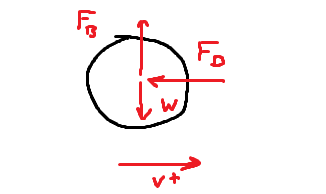
\includegraphics[width=0.6\textwidth]{Questions/Figures/Q3 FBD.png}
    \caption{Free body diagram of a sphere in a fluid.} 
    \label{fig:Q3 FBD}
\end{figure}

The frontal area of a sphere is $A = \pi D^2/4$. Substituting the expression for $F_D$ into the definition of $C_D$,
\begin{align*}
    C_D &= \frac{3\pi\mu VD}{\frac{1}{2}\rho V^2 \frac{\pi}{4} D^2} \\
    &= \frac{24\mu}{\rho VD}
    &= \boxed{\frac{24}{\text{Re}}}
\end{align*}
Since for Stokes flow, the Reynolds number is $\text{Re} \ll 1$, the drag coefficient will be very large.